
\chapter{Discussion}    
\label{Ch:Discussion}

%\citep{Antonny2016}
Recruitment and function of the Rvs complex in has been explored in this work, as well as several models for how membrane scission could be effected in yeast endocytosis. 
I propose that Rvs localizes to endocytic sites by interactions of the BAR domains of the Rvs complex with invaginated membrane, and that the SH3 domain mediated protein-protein interactions are required for efficient recruitment of Rvs to sites. Arrival of Rvs on membrane tube scaffolds the membrane and prevents premature membrane scission,till actin forces rupture the membrane, causing vesicle scission. Effective scaffolding depends on recruitment of a critical number of Rvs molecules. Here I discuss the main findings of this thesis in support of these propositions.



\section{Recruitment of Rvs to endocytic sites}
Rvs is relatively short-lived protein at endocytic sites. It is recruited only once membrane tube is formed (Kaksonen, Toret and Drubin, 2005; Kukulski et al., 2012; Picco et al., 2015). Fluorescence correlation spectroscopy (FCS) measurements have shown that the cytosolic concentration of Rvs167 and Rvs161 is quite high compared to other endocytic proteins (Boeke et al., 2014). Many endocytic proteins like Las17, Vrp1, type1 myosins, are measured at 80-240nM, while cytosolic concentration of Rvs161 and 167 is 721nM and 354nM respectively. In spite of this, relatively few numbers of Rvs are recruited to endocytic sites, suggesting that cytosolic concentration does not determine recruitment. Comparison between FCS measurements of cytoplasmic concentration for different endocytic proteins, and their recruitment to the endocytic sites indicates low correlation between the two, perhaps unsurprisingly, requiring that other directed mechanisms recruit proteins in a timed and efficient manner. In the case of Rvs, both timing and efficiency appear crucial to its function, the question is what confers both. 



%\subsection{Timing of localization and efficiency of recruitment}

\subsection{The BAR domain senses membrane curvature}
The curved structure of BAR dimers (Peter et al., 2004; Mim et al., 2012) has suggested that Rvs is recruited by its preference for some membrane shapes over others, supported by its arrival at curved membrane tubes. In the absence of membrane curvature, in \textit{sla2$\Delta$} cells, the BAR domain alone does not localize to cortical patches (Fig.\ref{delsh3_latA}D). This demonstrates for the first time that the BAR domain does indeed sense and requires membrane curvature to localize to cortical patches. Work on BAR domains have proposed that electrostatic interactions between positive charges at the concave surface and tips of the BAR domain structure and negatively charged lipids mediate membrane binding(Qualmann, Koch and Kessels, 2011). Mutations in these lipid-binding surfaces would clarify the interaction with underlying lipids, and test if Rvs relies on similar interactions.



\subsection{BAR domain times recruitment of Rvs} 

BAR is able to localize to endocytic sites, and has a similar lifetime in WT cells (Fig.\ref{delsh3_latA}, Fig.\ref{delsh3_movement}). In Fig.\ref{disc_concentration}B,D we see that while the full-length Rvs167 arrives about 4 seconds after the arrival of Abp1, BAR arrives only 6 seconds after Abp1 arrives. There is a time delay between Abp1 recruitment and BAR arrival, compared to the arrival of full-length Rvs167, confirmed by the TIRF measurement in \ref{disc_concentration}D. 

	\vspace{5mm}
The delay in recruitment could occur because the membrane has not acquired the required invagination length or because the loss of the SH3 domain causes delayed recruitment. That the delayed recruitment occurs because the invagination takes longer to reach a particular length is supported by the fact that Sla1 moves inwards at a slower rate in BAR cells. It takes longer for the membrane in BAR cells to reach the same length as WT. Rvs167 arrives in BAR cells when Sla1 has moved inwards 25-30nm (dashed red lines in Fig.\ref{delsh3_latA}A), which is also the distance Sla1 has moved when Rvs167 arrives in WT. By the time Sla1 has moved this distance, the membrane is already tubular (Kukulski et al., 2012; Picco et al., 2015), consistent with Rvs arrival at invaginated tubes. This suggests Rvs recruitment is timed to specific membrane invagination length- therefore to a specific membrane curvature- and that this timing is provided by the BAR domain. 



\subsection{The SH3 domain makes Rvs recruitment efficient} 
As seen in Fig.\ref{delsh3_latA}C, Rvs167 in BAR cells accumulates to about half the WT number, even though the same cytoplasmic concentration is measured. This indicates that the SH3 domain increases the efficiency of recruitment of Rvs. Either SH3 domain helps recruitment to endocytic sites, or it stabilizes interaction with sites. In \textit{sla2$\Delta$}  cells, full-length Rvs can assemble on the membrane (Fig.\ref{delsh3_latA}D-F). Since BAR domains alone do not localize to patches in \textit{sla2$\Delta$}  cells, full-length localization must be mediated by the SH3 domain, supporting a role for the SH3 domain in increasing recruitment of Rvs by clustering protein molecules. 


\subsection{The SH3 domain can assemble and disassemble Rvs molecules independent of the BAR domain and actin interactions} 
As mentioned above, in \textit{sla2$\Delta$}  cells, full-length Rvs167 is able to assemble and disassemble at cortical patches without the curvature-dependent interaction of the BAR domain (Fig\ref{delsh3_latA}D-F). This unexpected finding indicates that the SH3 domain is able to mediate both the recruitment and then disassembly of Rvs at the endocytic site. 


	\vspace{5mm}
In \textit{sla2$\Delta$}  cells treated with LatA (Fig.\ref{delsh3_latA}G-H), actin-based membrane curvature is inhibited, and the actin patch proteins are removed from the plasma membrane. Full-length Rvs167 in these cells still shows transient localizations at the plasma membrane (Fig.\ref{delsh3_latA}A). In \textit{sla2$\Delta$}  cells treated with LatA, the localization of BAR is lost, suggesting that its localization is dependent on an SH3 domain interaction, and that this is independent of both actin and membrane curvature. 


\subsection{SH3 domain affects actin dynamics}
In WT cells, the Abp1 and Rvs167 fluorescent intensities reach maxima concomitantly, and the consequent decay of both also coincide. That this occurs at the same time indicates that upon vesicle scission, the actin network is immediately disassembled. Membrane scission essentially occurs around the intensity peak of the two proteins. This coincident peak is lost in BAR cells. Rvs in these cells peaks several seconds after Abp1 intensity starts to drop, and the decay of Abp1 is prolonged, taking nearly double the time as in WT. As we see in Fig.\ref{delsh3_movement}C, the number of Abp1 molecules recruited is decreased to about two thirds the WT number. Although it is not clear what the decoupling of Abp1 and Rvs peaks means, the changes in Abp1 dynamics suggests a strong disruption of the actin network. SH3 domains are known to interact with components of the actin network like Abp1 and Las17 (Lila and Drubin, 1997, Madania et al., 1999), but study of other components of the actin machinery will be required to understand how exactly loss of the SH3 has changed the progression of endocytosis.  


\subsection{What does the SH3 domain interact with?}
SH3 interaction with an endocytic binding partner could help recruit Rvs to endocytic sites. Many such interaction partners have been proposed. Abp1 interaction with the Rvs167 SH3 domain has been shown (Lila and Drubin, 1997; Colwill et al., 1999), as has one with WASP protein Las17 (Madania et al., 1999; Liu et al., 2009), yeast Calmodulin Cmd1 (Myers et al., 2016), type I myosins (Geli et al., 2000), and Vrp1 (Lila and Drubin, 1997). These proteins are currently being studied as potential targets of the Rvs167 SH3 domain. All of these suggested binding partners localize to the base of the invagination (Yidi Sun, 2006; Picco et al., 2015), and do not follow the invaginating membrane into the cytoplasm. If one of these is the SH3 interaction partner, SH3 domains interact with the endocytic network at the base of the invagination. Centroid tracking however, suggests that Rvs is accumulated all over the membrane tube without bias towards the base of the invagination. If Rvs was recruited to the base and pulled up as the invagination grows, the centroid would move continuously upwards rather than remain relatively non-motile before the jump at scission time. It is possible that the SH3 initially helps cluster near the base, and as the membrane invaginations grow longer, BAR-membrane interactions dominate. 





\subsection{Total number of Rvs recruited is independent of ploidy}
When ploidy is doubled from haploids to diploids, we could expect that double the protein amount is expressed and recruited, but it does not appear so. The amount of Rvs recruited in WT haploid (1xh) and diploids (2xd) remains about the same, and cytoplasmic signal is similar (Fig.\ref{disc_concentration}). This invariance between accumulated protein in haploids and diploids shows that Rvs recruitment is not determined by the number of alleles of Rvs. Haploid and diploid cells appear to tune the amount of Rvs recruitment to get a specific amount to endocytic sites.

	\begin{figure}[H]
	\centering
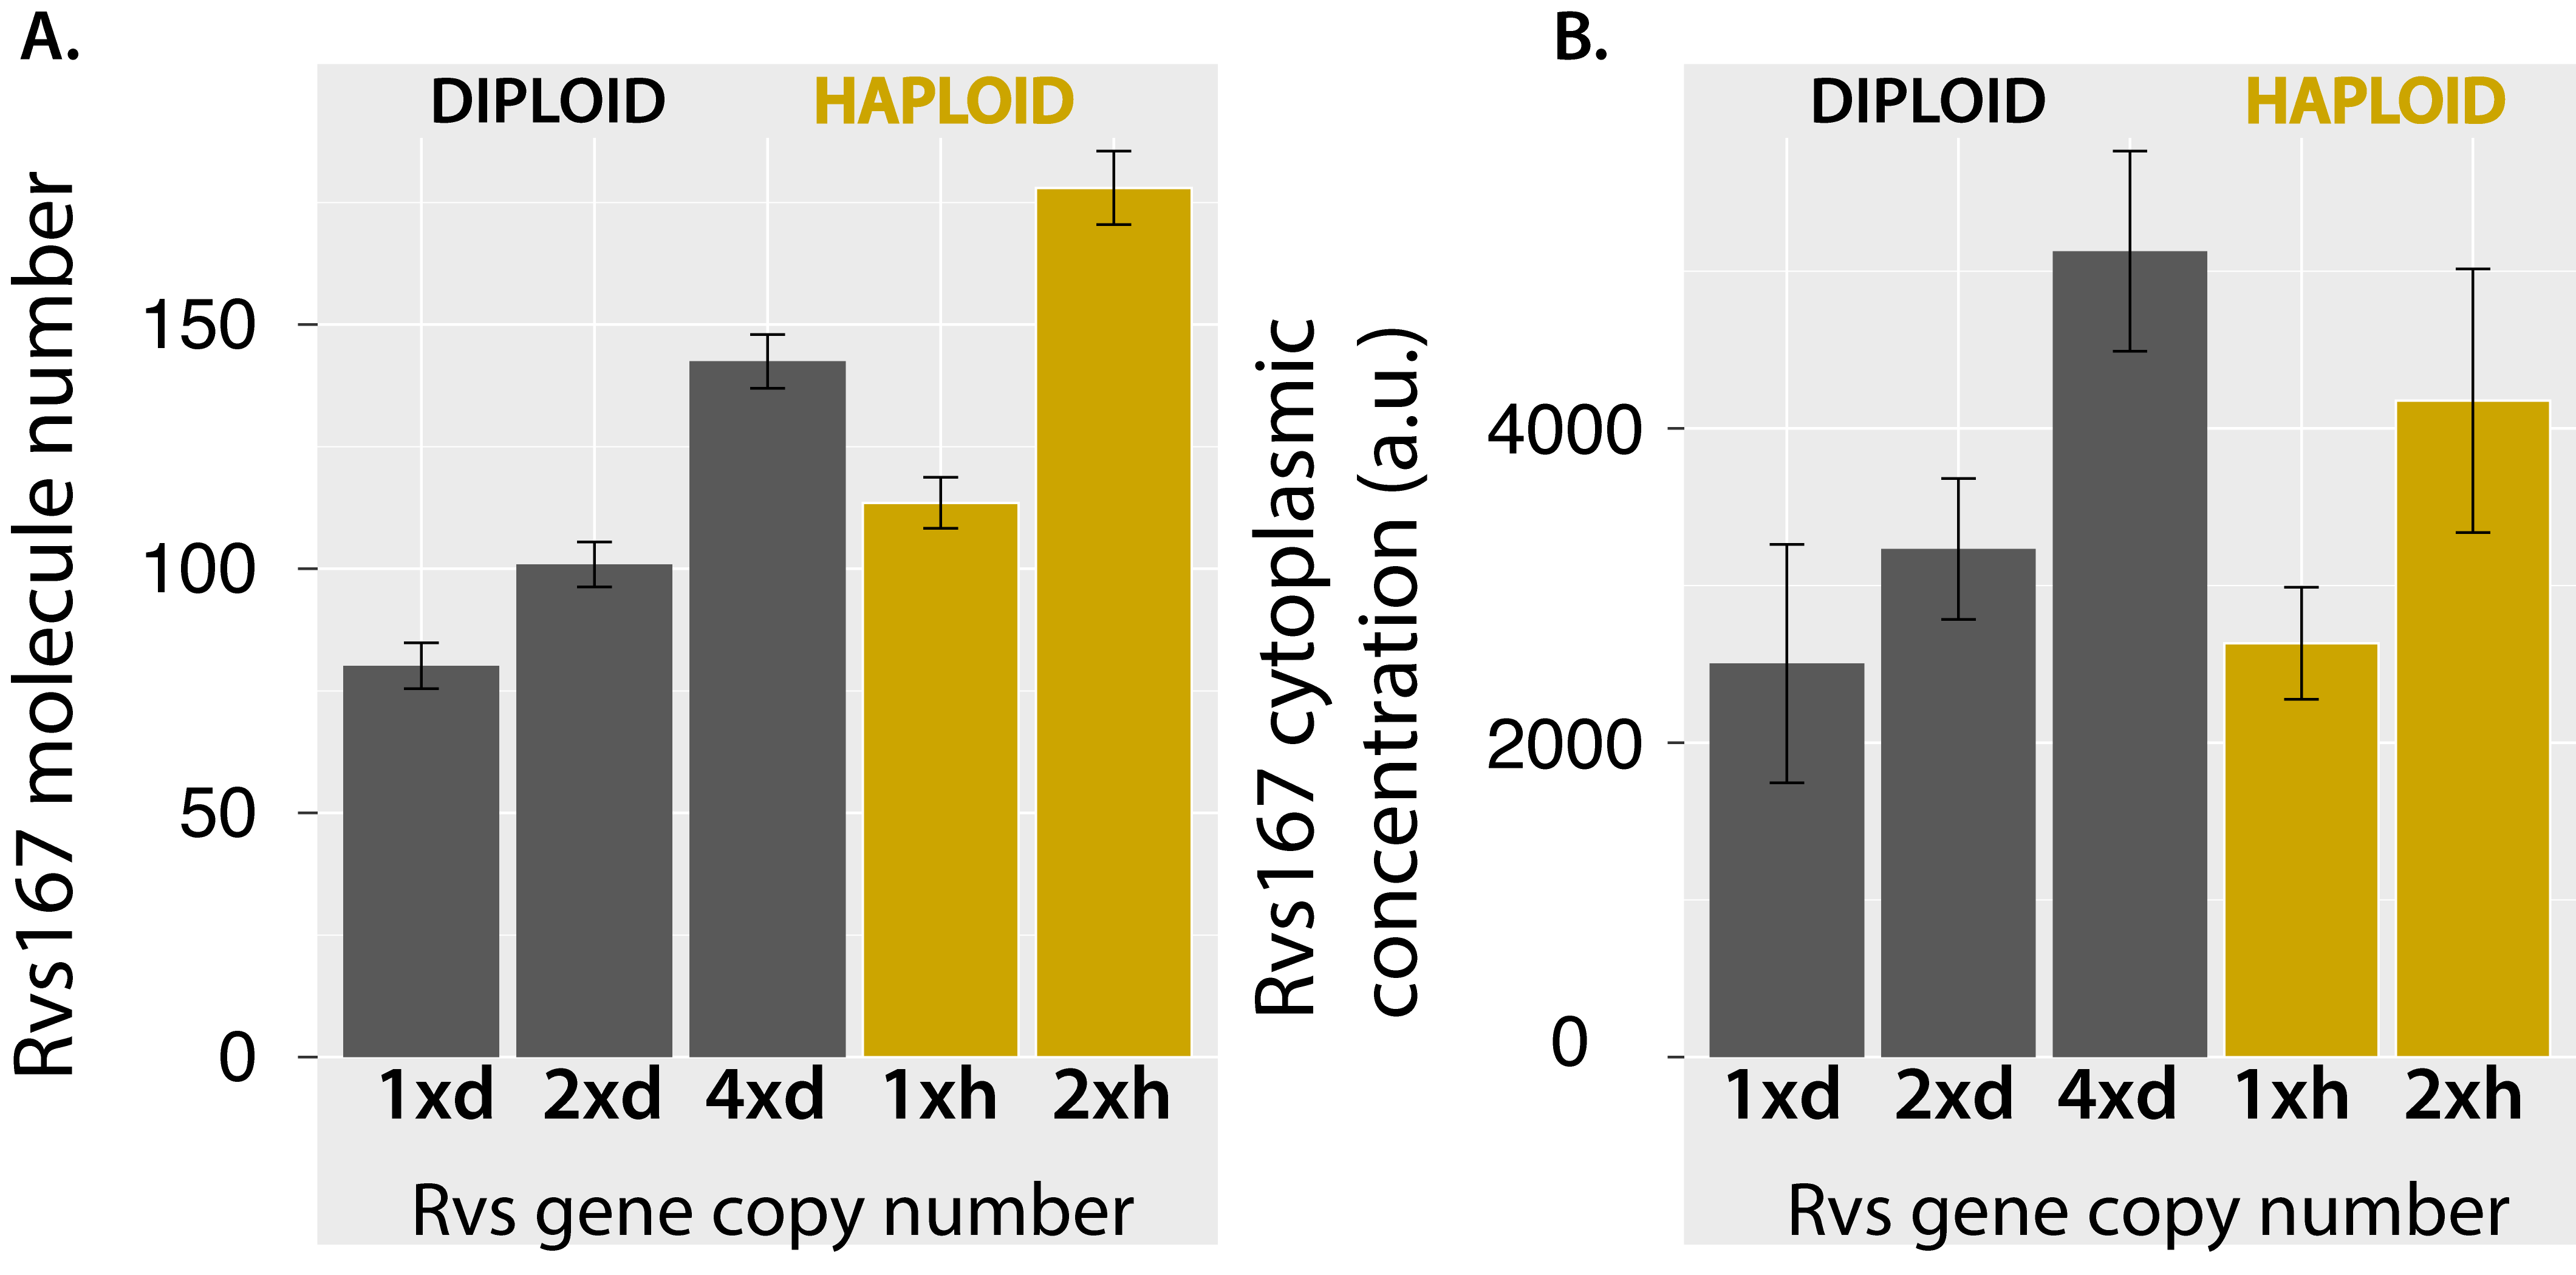
\includegraphics[width=11cm,height=12cm,keepaspectratio]{figures/discussion/number_comp}
	\caption[Recruitment of Rvs]
	{A. Maximum molecule number of Rvs167-GFP recruited with S.E.M in haploid and diploid cells with different gene copies of Rvs. 
	B. Cytoplasmic signal of Rvs167-GFP with standard deviation in haploid and diploid cells with different gene copies of Rvs. 
	\label{disc_concentration}}
	\end{figure}
%	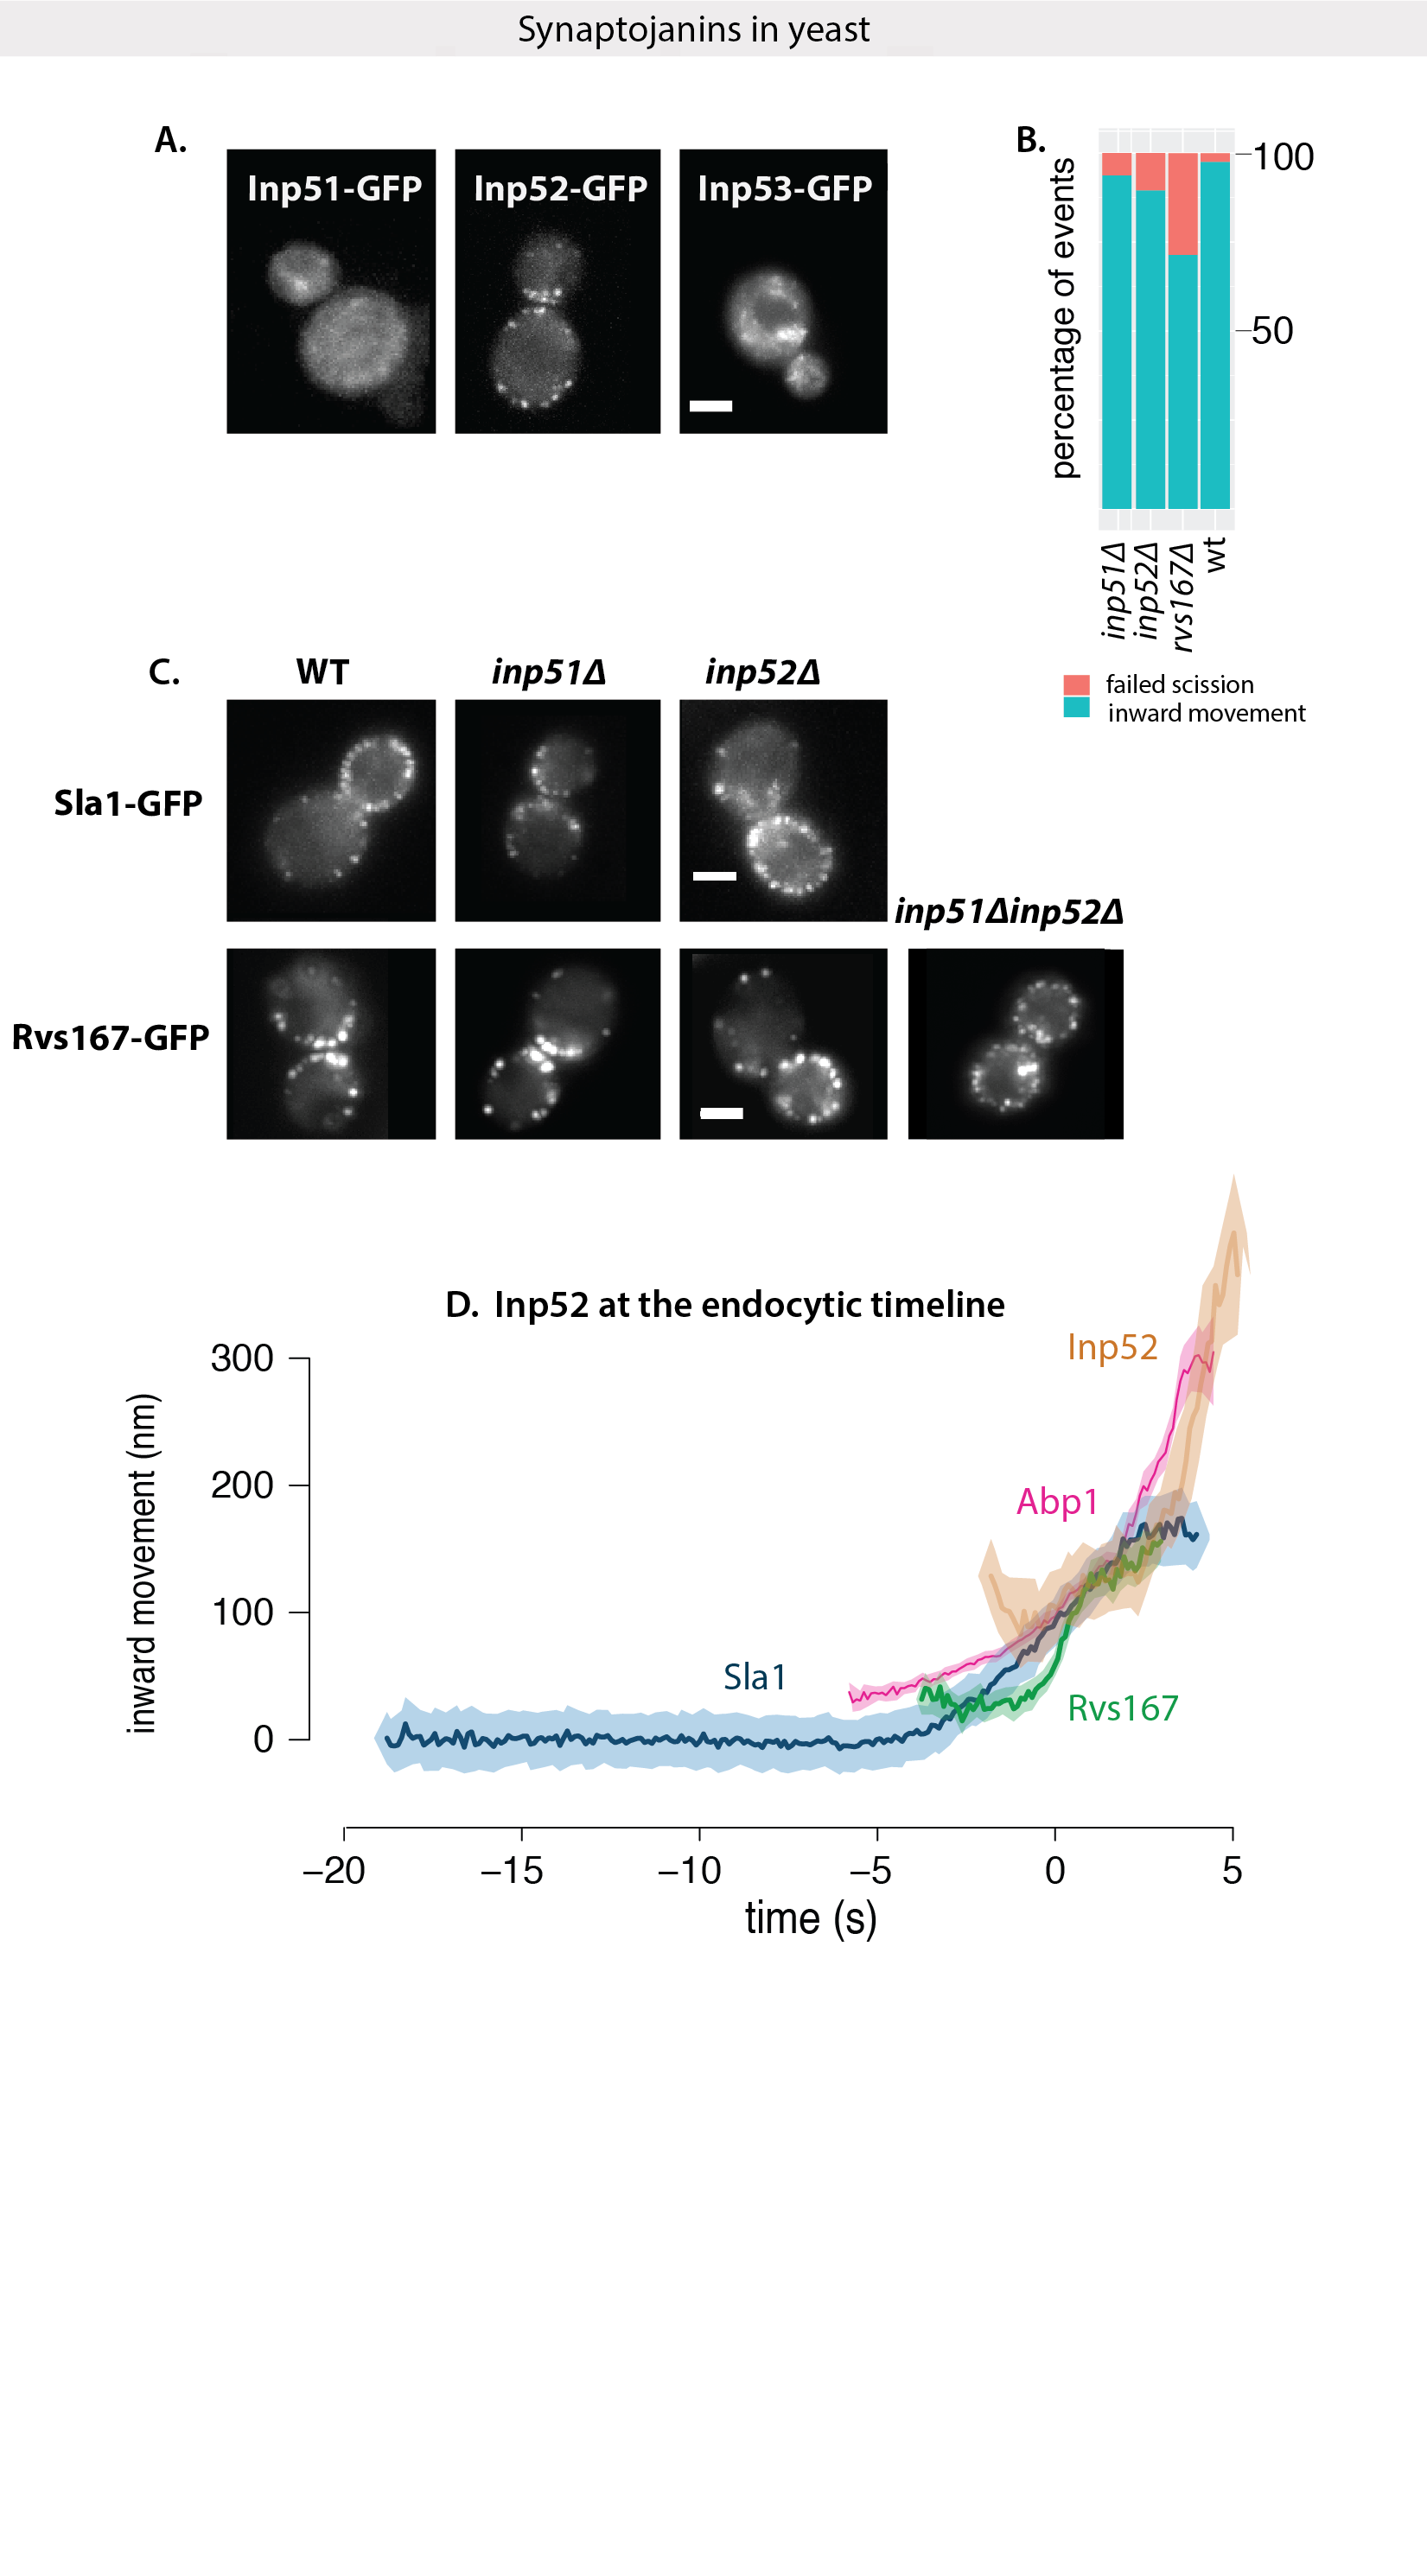
\includegraphics[width=19cm,height=19cm,keepaspectratio]{figures/results_final/inp}

\subsection{Rvs recruitment rate increases with increasing gene copy number}
WT diploid cells (2xd) contain two copies each of Rvs161 and Rvs167. Rvs duplicated diploids, which contain four copies each of Rvs167 and Rvs161 (4xd) could be expected to express and recruit to sites twice the amount of Rvs as 2xd. However, compared to 2xd, cytoplasmic signal in 4xd increases by 1.6x and recruitment of Rvs167 to endocytic sites increases only by 1.4x. Doubling the gene copy number increases, but does not double protein expression or recruitment in the case of Rvs. Similarly, duplicating Rvs genes in haploid cells results in an increase in number of molecules recruited, but not in doubling (1xh, 2xh). Although the rate of adding Rvs is different in haploids and diploids, in both cases, it increases by gene copy number (yellow line in Fig.\ref{disc_recruit_rate}). 

	\begin{figure}[H]
	\centering
	\hspace{-1cm}
	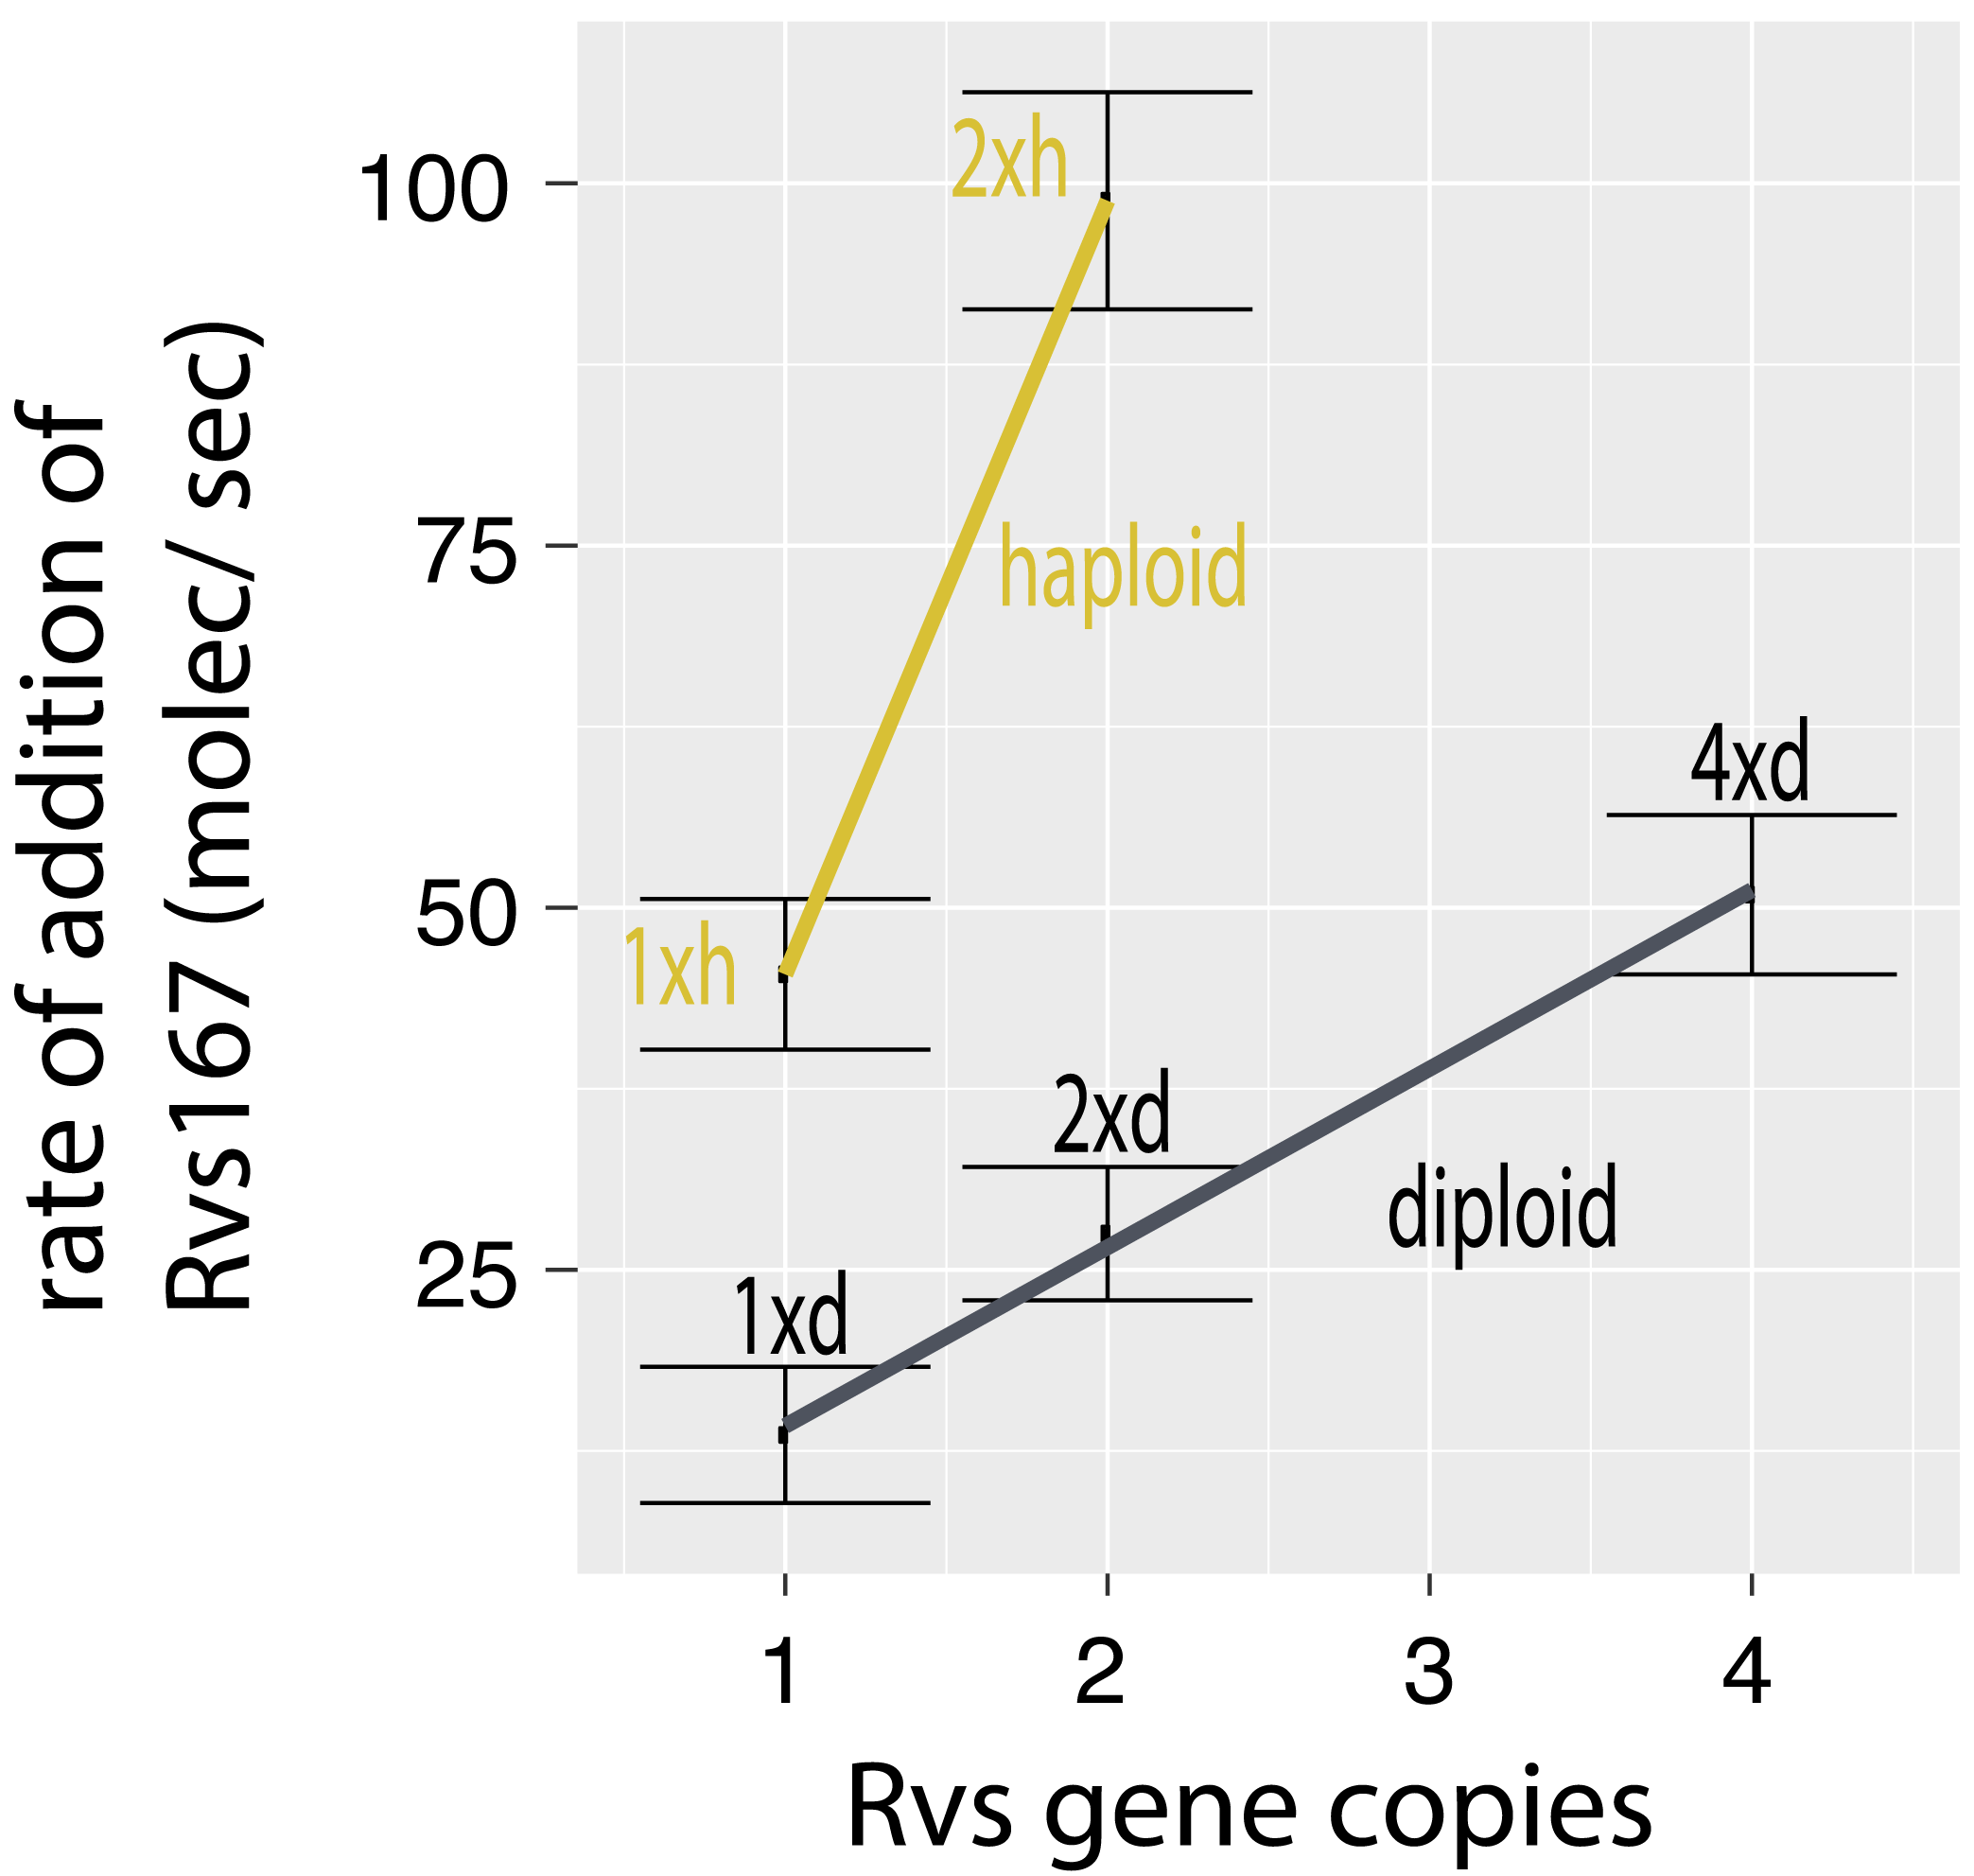
\includegraphics[width=8cm,height=8cm,keepaspectratio]{figures/discussion/recruit_rate_final}
	\caption[Rate of recruitment of Rvs]
{Rate of Rvs molecules added to endocytic sites before scission vs gene copy number in haploids and diploids. SEM of the molecule numbers recruited, and linear fit through the data is shown.
	\label{disc_recruit_rate}}
\end{figure}

	\vspace{5mm}
When haploid and diploid data are considered separately, cytoplasmic protein concentration is increased when gene copies are increased, and recruitment to endocytic sites is increased by the increase in cytoplasmic concentration. These data suggest that the amount of Rvs that is recruited scales with available concentration of protein. Comparing across ploidy however, the rate of Rvs recruitment is lower in WT diploid compared to WT haploid (2xd vs 1xh, Fig.\ref{disc_concentration}) in spite of the same cytosolic concentration of Rvs in both. The reason for this is not clear. 


%	\vspace{5mm}
%Cytoplasmic protein concentration is increased when gene copies are increased, and recruitment to endocytic sites is increased by the increase in cytoplasmic concentration. Although this data needs to be confirmed by quantitative western blots for protein expression, it suggests that how much Rvs is recruited scales with available concentration of protein. 



\section{Arrangement of Rvs dimers on the membrane}
A homology model of the Rvs BAR dimer structure based on Amphiphysin suggests that it has the typical concave structure typical for N-BAR domains. Rvs is a hetero- rather than homodimer however, and a high-resolution detail will be necessary to clarify the interaction and arrangement of Rvs on endocytic tubes. It is therefore unclear how Rvs is arranged, although there are some indications from the experiments in this thesis of the interaction with the membrane.



\subsection{Rvs does not form a tight scaffold on membrane tubes}
\textit{In vitro} helices of BAR domains have suggested that Rvs might form a similar helical scaffold. The number of Rvs molecules recruited to endocytic sites is high enough to cover the surface area of the tubular invagination, so it has been proposed that an Rvs scaffold covers the entire membrane tube up to the base of the future vesicle (Picco et al., 2015). 

	\vspace{5mm}
In Rvs duplicated diploid cells (4xd), Rvs can be recruited at a much faster rate than in than in the WT (2xd) (Fig.\ref{fig_rvsdiploid1}B-C, Fig.\ref{disc_recruit_rate}) while disassembly dynamics is the same in both (Fig.\ref{fig_rvsdiploid1}C, Fig.\ref{disc_decay}). The exponential decay of fluorescent intensity in WT haploid and diploid cells (1xh, 2xd, Fig.\ref{disc_decay}) indicates that all of the protein is suddenly disassembled from the endocytic site. When the membrane tube undergoes scission, there is no more tubular curvature for the Rvs to bind to. The sharp decay is therefore consistent with a BAR scaffold that breaks upon vesicle scission because there is no more membrane interaction, releasing all the membrane-bound protein at once. 



	\vspace{5mm}
A similar decay in the 4xd strain suggests that all the Rvs in this case is also bound to the membrane: if the protein was not bound to the membrane, fluorescent intensity would not decay sharply. Since the membrane is able to accommodate 1.4x the amount of BAR protein as the WT, it would suggest that at lower protein amounts, a tight helix that covers the entire tube is not likely. Adding molecules to a tube already completely covered by a scaffold would result in a change in Rvs assembly and disassembly dynamics. 

Further, additional molecules would have to be added at the top or base of a tight scaffold. At the top, the radius of curvature is decreased compared to the tube since this is the rounded vesicle region. At the base, the plasma membrane is nearly flat, and the Rvs BAR domain is similarly unlikely to favour interactions here. Otherwise the scaffold would have to be disrupted to add new molecules, which would likely slow down recruitment rate rather than speed it up. Molecules could also be added concentric to an existing scaffold. The concave surface of Rvs is known to interact with lipids, and multiple layers of BAR domains on the membrane tube would probably not show the sudden disassembly seen here.  

I assume that the membrane surface area does not change in the 4xd compared to 2xd from the identical movement of Sla1 in both cases (Fig.\ref{fig_rvsdiploid1}A). It is possible that a wider tube is formed, which would increase the membrane surface area for BAR binding. This would, however, require the BAR domains to interact with a lower radius of curvature than in WT. This seems unlikely, and in the absence of any indication otherwise, I assume that the membrane tubes in all diploid and haploid cases have the same width.


\subsection{A limit for how much Rvs can be recruited to the membrane}
In the case of Rvs duplication in haploids (2xh), a change in disassembly dynamics is seen (Fig.\ref{fig_rvshaploid}B, Fig.\ref{disc_decay}). In 2xh, the maximum number of molecules recruited is 178$\pm$7.5 compared to the maximum of 113.505$\pm$5.2 in WT (1xh). This is means that nearly 1.6x the WT amount of protein is recruited to membrane tubes in in the 2xh case. The Rvs167 fluorescent intensity in 2xh shows a delay in disassembly. This suggests that the excess protein may not be directly on the membrane, since if the protein was membrane bound, when the membrane breaks, the protein must be released. The excess Rvs could either interact with the actin network via the SH3 domain, or interact with other Rvs dimers. By a similar argument as 4.2.1 above, I do not expect that multiple layers of BAR domains are formed, and that the excess protein is recruited by the interaction of the SH3 domain. 


	\vspace{5mm}
Another explanation for the delayed disassembly is that at high concentrations of Rvs in the 2xh case, a tight BAR scaffold is formed, and the BAR domains interact with each other. When the membrane undergoes scission, the protein is no longer membrane bound, but lateral interactions delay disassembly of the scaffold. Lateral interactions between adjacent BAR dimers have been shown in the case of Endophilin  (Mim et al., 2012). It is not currently clear where the Rvs molecules are added in the 2xh case: supperresolution microscopy could clarify whether it is added at the membrane tube.

\vspace{5mm}
Whatever the arrangement of the Rvs complex on the membrane, disassembly dynamics is changed in the case of 2xh, compared to all the other haploid and diploid strains. Since the number of Rvs molecules is highest in this strain, this suggests that there is a limit to how much Rvs can assemble on the tube without altering interaction with the endocytic protein network. 

\begin{figure}[H]
	\centering
	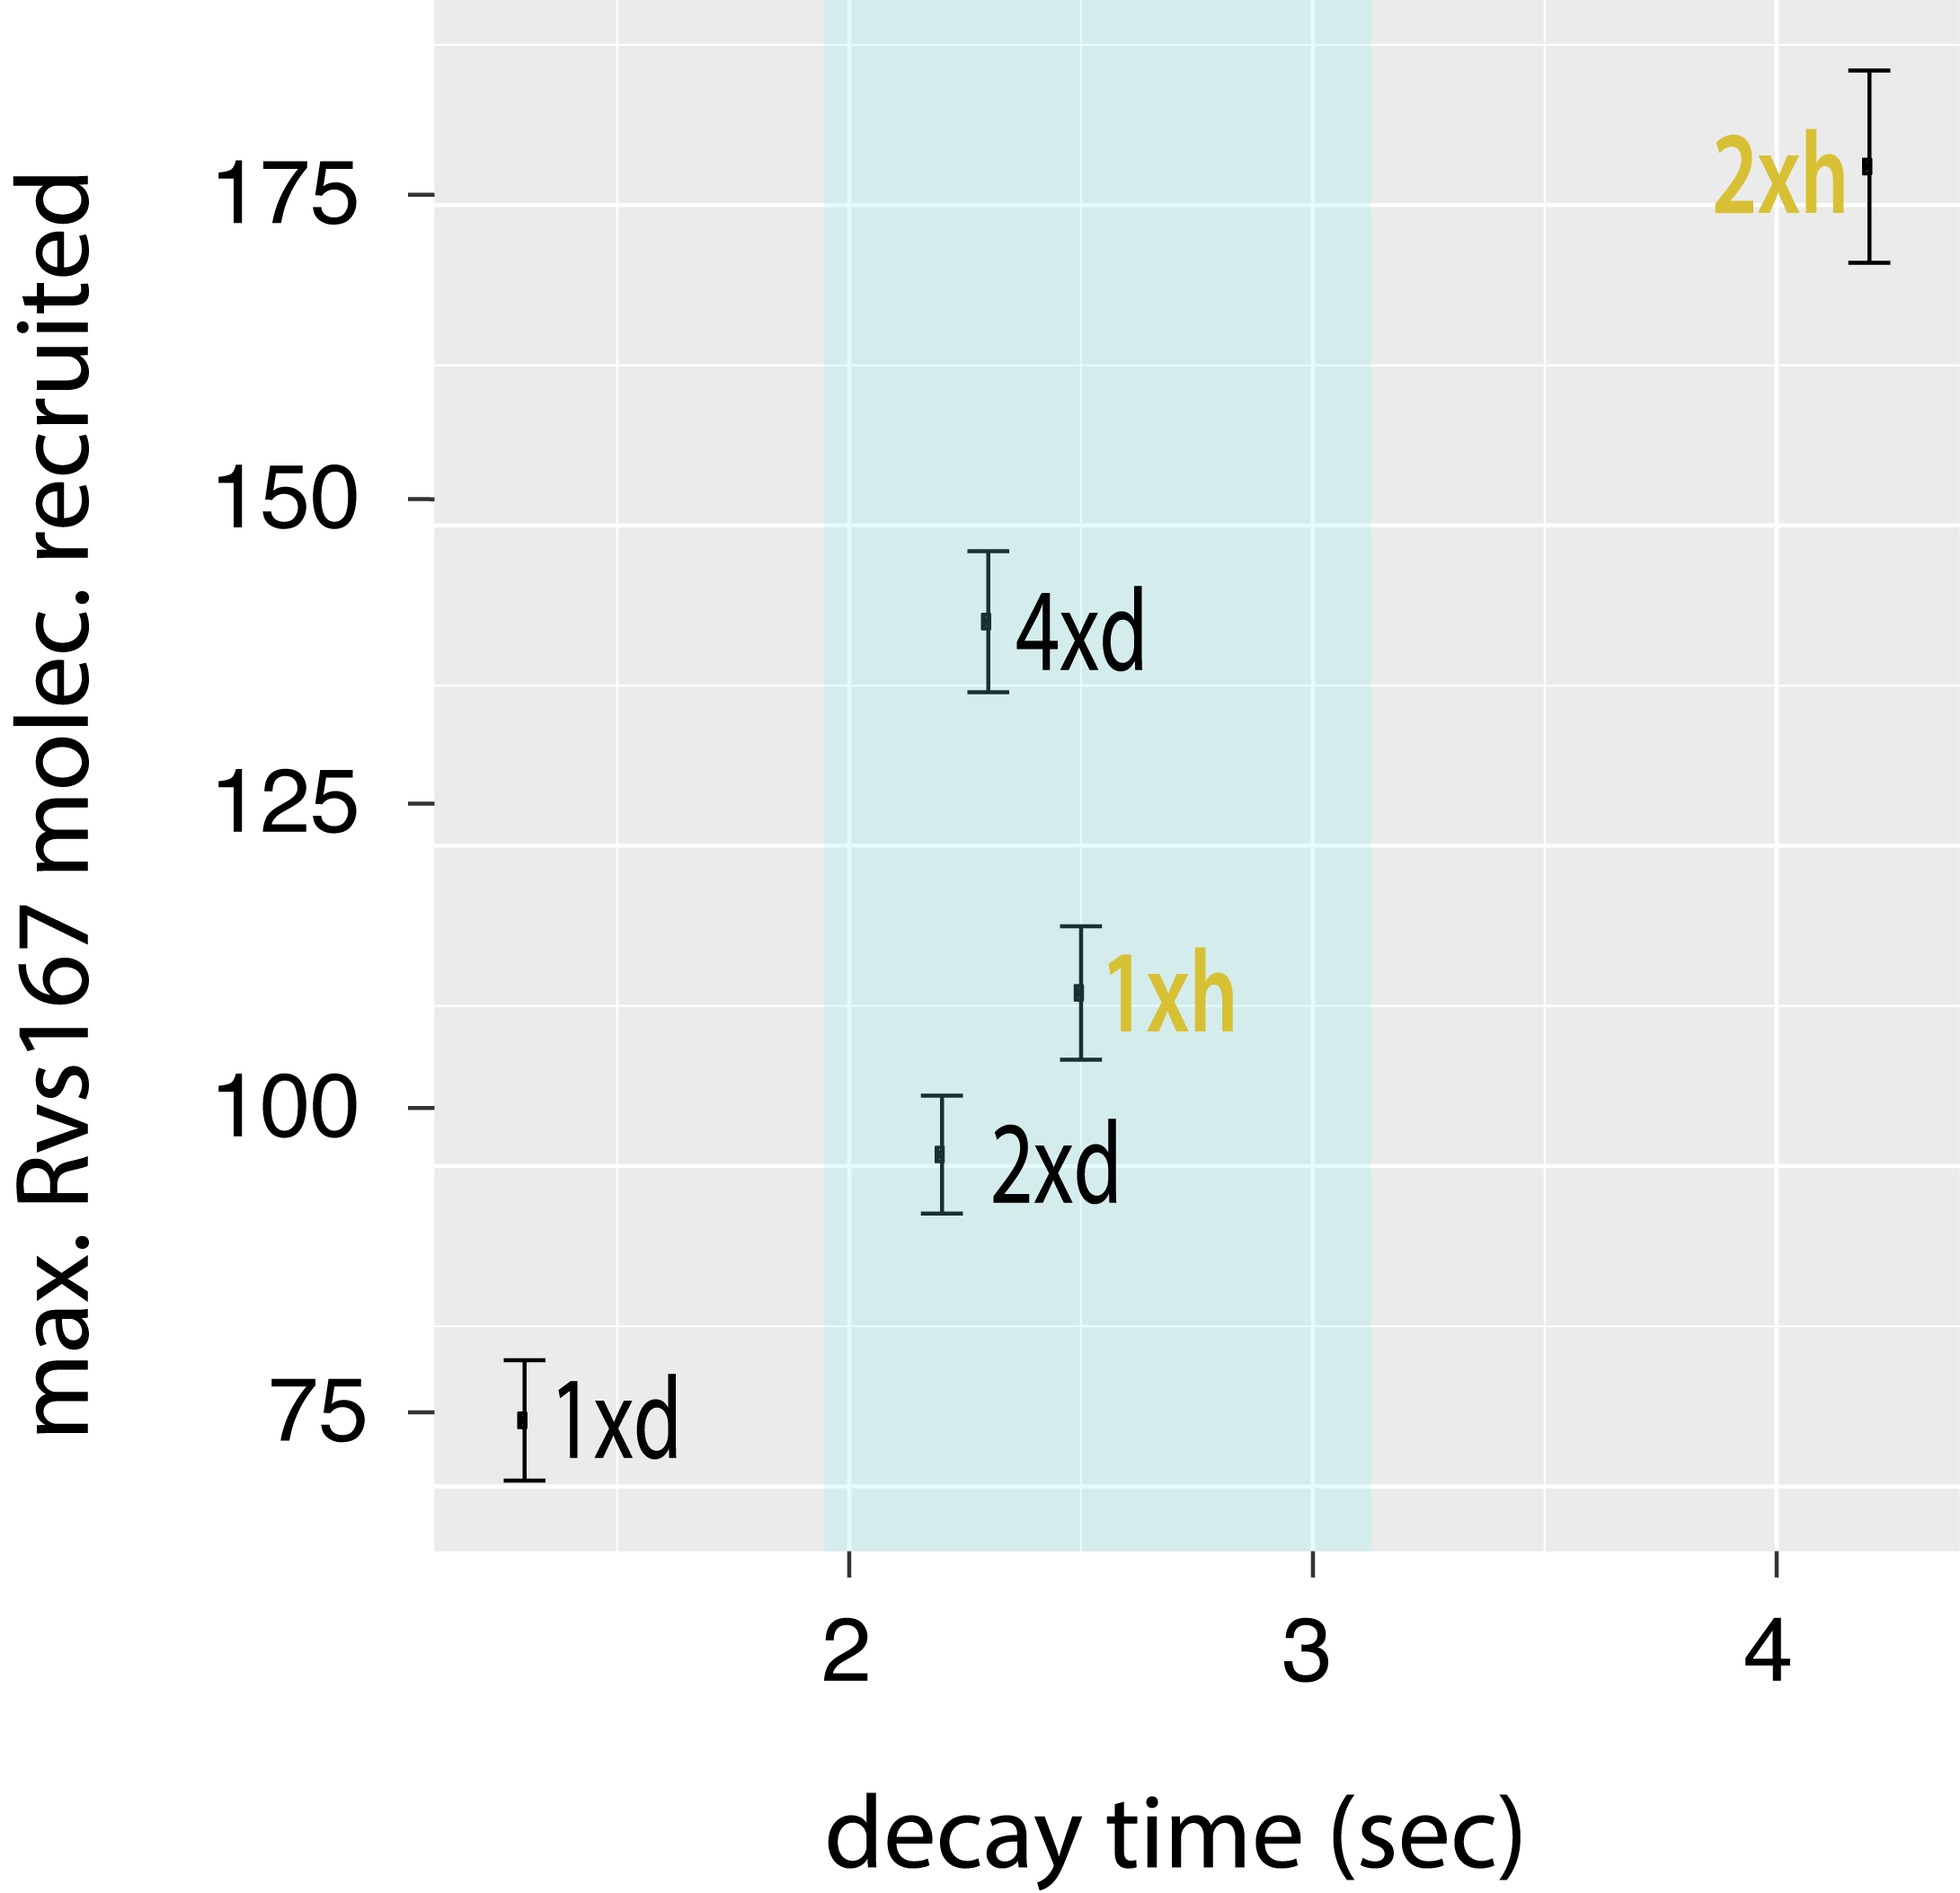
\includegraphics[width=9cm,height=9cm,keepaspectratio]{figures/discussion/decay_final}
	\caption[Rvs decay time]
	{Time from peak of Rvs fluorescent intensity to minimum intensity, against maximum molecule numbers recruited. Coloured region highlights similar disassembly time for increasing amounts of molecules recruited.    
		\label{disc_decay}}
\end{figure}

\subsection{Conclusions for Rvs localization }
All of these data support the idea that Rvs recruitment rate and total numbers are determined by concentration of protein in the cell. The maximum number of molecules can interact with the membrane is limited by the membrane surface area of the invagination tube. Although more can be recruited, Rvs over a certain threshold concentration interacts in a different way with endocytic sites, likely via the SH3 domain. Timing of recruitment to sites is by curvature-recognition via the BAR domain, while efficiency of recruitment and interaction with the actin network is established via the SH3 domain. 



\section{What causes membrane scission?}


\subsection{Dynamin does not not drive scission}
Some studies have suggested that dynamin-like Vps1 localizes to endoytic sites, and affects the scission mechanism: Nannapaneni et al(Nannapaneni et al., 2010)., find that the lifetimes of Las17, Sla1, Abp1 increase in the absence of Vps1. Rooij et al (Rooij et al., 2010)., find that Rvs167 lifetimes increase, and are recruited in fewer patches to the cell cortex. On the other hand, \textit{vps1$\Delta$} did not increase the scission failure rate of \textit{rvs167$\Delta$} in other studies (Kishimoto et al., 2011), and did not co-localize with endocytic proteins (Goud Gadila et al., 2017). If Vps1 was to affect scission, the number of failed scission events should increase in \textit{vps1$\Delta$} cells, but I do not find so, confirming other studies (Kishimoto et al., 2011). Vps1 tagged with GFP and imaged in TIRF does not form cortical patches that co-localize with Abp1-mCherry (data from Andrea Picco, not shown). GFP-tagging could affect the recruitment of Vps1 to endocytic sites while maintaining its role in other pathways of vesicular trafficking. Membrane movement and scission dynamics are however, unchanged in the absence of Vps1. If loss of Vps1 prevented or delayed scission, the membrane would continue to invaginate longer than WT lengths, and Sla1 movements of over 140nm should be observed. Rvs centroid movement would likely also be affected: a bigger jump inwards could indicate that that a longer membrane has been cut. My observation that there are no changes in the behaviour of coat and scission markers indicates that even if Vps1 is recruited to endocytic sites, it is not necessary for Rvs localization or function, and is not necessary for scission. 



\subsection{Lipid hydrolysis is not the primary cause of membrane scission}
In this model, synaptojanins hydrolyze 	PIP\textsubscript{2} that are not covered by BAR domains, resulting in a boundary between hydrolyzed and non-hydroplyzed 	PIP\textsubscript{2} The model predicts that interfacial forces generated at the lipid boundary causes scission (Liu et al., 2006).  Inp52 localizes to the top of invaginations right before scission, consistent with a role in vesicle formation (Fig.\ref{fig_inp}). Synaptojanin-like Inp51 is not seen to localize to the cellular cortex, but this could indicate that protein recruitment to the endocytic patches is below our detection limit. 


\vspace{5mm}

First, vesicle scission is expected to occur at the interphase of the hydrolyzed and non-hydrolyzed lipid. Since the BAR scaffold covers the membrane tube, this interphase would be at the top of the area covered by Rvs. Kukulski et al. (Kukulski et al. 2012) have shown that vesicles undergo scission at 1/3 the invagination length from the base: that is, vesicles generated by the lipid boundary would be smaller than have been measured. Second, removing forces generated by lipid hydrolysis by deleting synaptojanins should increase invagination lengths, since scission would be delayed or fail without those forces. Deletion of Inp51 and Inp52 does not change the invagination lengths: Sla1 movement does not increase. That the position of the vesicle formed is also unchanged compared to WT is indicated by the magnitude of the jump into the cytoplasm of the Rvs centroid. 

\vspace{5mm}

First, vesicle scission is expected to occur at the interphase of the hydrolyzed and non-hydrolyzed lipid. Since the BAR scaffold covers the membrane tube, this interphase would be at the top of the area covered by Rvs. Kukulski et al. (Kukulski et al., 2012) have shown that vesicles undergo scission at 1/3 the invagination length from the base: that is, vesicles generated by the lipid boundary would be smaller than have been measured. Second, removing forces generated by lipid hydrolysis by deleting synaptojanins should increase invagination lengths, since scission would be delayed or it would fail without those forces. Deletion of neither Inp51 nor Inp52 changes the invagination lengths: Sla1 movement does not increase. That the position of the vesicle formed is also unchanged compared to WT is indicated by the magnitude of the jump into the cytoplasm of the Rvs centroid. 


\vspace{5mm}
There are some changes in the synaptojanin deletion strains. In \textit{inp51$\Delta$} cells, Rvs assembly is slightly slower than that in WT. Therefore, Inp51 could play a role in Rvs recruitment. In the \textit{inp52$\Delta$} strain, about 12\% of Sla1-GFP tracks retract, indicated that scission fails in those cases. Although this is low compared to the failed scission rate of \textit{rvs167$\Delta$} cells (close to 30\%), this data could suggest a moderate influence of Inp52 on scission. Rvs centroid persists after scission for about a second longer in \textit{inp52$\Delta$} cells than in WT, indicating that disassembly of Rvs on the base of the newly formed vesicle is delayed.

\vspace{5mm}
In \textit{inp51$\Delta$}\textit{inp52$\Delta$} cells, Rvs is accumulated at patches, but majority of Rvs patches do not show the typical sharp jump into the cytoplasm. Membrane morphology is hugely aberrant in these cells, complicating interpretation of this data (Srinivasan et al., 1997). Electron microscopy shows long, undulating membrane invaginations Srinivasan et al., 1997. Fluorescence microscopy shows that multiple endocytic sites that are assembled and disassembled at these long invaginations, and fail to undergo scission ( Sun et al., 2007). Where on these long membranes Rvs localizes could be clarified by CLEM or super-resolution microscopy. Large clusters of Rvs seen in the \textit{inp51$\Delta$}\textit{inp52$\Delta$} strain could be multiple Rvs patches on same membrane tube. Pooling signal from multiple endocytic sites would influence the molecule numbers acquired by our analysis, and yield a higher number than at a single site. Rvs does, interestingly, assemble and disassemble in these mutants. If no vesicles are formed at these membranes, it would indicate that Rvs disassembly is not caused by membrane scission.


\subsection{Protein friction does not drive membrane scission}
Protein-friction mediated membrane scission proposes that BAR domains induce a frictional force on the membrane, causing scission. In Rvs duplicated haploid cells (2xh), adding up to 1.6x the WT (1xh) amount of Rvs to membrane tubes does not affect the length at which the membrane undergoes scission (Fig.\ref{fig_rvshaploid}). The model introduced in Section 3.4.3 predicts that if more BAR domains were added to the membrane tube, frictional force generated as the membrane is pulled under it will increase, and the membrane would rupture faster. That is, membrane scission occurs as soon as WT forces are generated on the tube. Since BAR domains are added at a faster rate in the 2xh cells, these forces would be reached at shorter invagination lengths. In 2xh cells, WT amount of Rvs is recruited at about 1.8 seconds before maximum fluorescent intensity, but scission does not occur at this time. Instead, Rvs continues to accumulate, and the invagination continues to grow. In diploid strains, adding 1.4x the WT amount of Rvs in the 4x Rvs case also does not change length of membrane that undergoes scission. Therefore, protein friction due to Rvs does not appear to contribute significantly to membrane scission in yeast endocytosis. 


\subsection{ Actin polymerization generates forces required for membrane scission}
Maximum amount of Abp1 measured in all the diploid strains is about 220 molecules (Fig.\ref{fig_rvsdiploid2}). In this case, only one allele of Abp1 is fluorescently tagged, so half the amount of Abp1 recruited is measured. The maximum amount of Abp1 recruited is then double that measured, which is about 440$\pm$20 molecules (assuming equal expression and recruitment of tagged and untagged Abp1). In WT haploid cells, the maximum number of Abp1 measured is 460$\pm$20 molecules. That the same number of molecules of Abp1 is recruited in all cases before scission indicates that scission timing depends on the amount of Abp1, and hence, on the amount of actin recruited. 

\vspace{5mm}
This data is consistent with actin supplying the forces necessary for membrane scission. The membrane invagination continues until the “right” amount of actin is recruited. At this amount of actin, enough forces are generated to rupture the membrane. The amount of force necessary is determined by the physical properties of the membrane like membrane rigidity, tension, and proteins accumulated on the membrane (Dmitrieff and Nédélec, 2015). Vesicle scission releases membrane-bound Rvs, resulting in release of the SH3 along with BAR domains. Release of the SH3 domains could indicate to its binding partner in actin network that vesicle scission has occurred, beginning disassembly of actin components. In the BAR strains, a low amount of actin is recruited (Fig.\ref{fig2_sh3del}C). It is clear that in the absence of the SH3 domain, the actin network is severely perturbed, and the effect of this on scission dynamics is currently unclear. 

\section{Function of the Rvs complex}

\subsection{Rvs scaffolds membrane pore}
Sla1 in \textit{rvs167$\Delta$} cells undergoes scission at short invagination lengths of about 60nm (Fig.\ref{fig2_rvsdelta}), compared to the WT lengths of 140nm. This shows that first, enough forces are generated at 60nm to cause scission. Then, that Rvs167 is required at membrane tubes to prevent premature scission. 

Prevention of scission at short invagination lengths can be explained by Rvs stabilizing the membrane invagination via membrane interactions of the BAR domain (Boucrot et al., 2012; Dmitrieff and Nédélec, 2015). Rvs preventing membrane scission could be explained by the SH3 domain mediating actin forces to the invagination neck: one can imagine that the SH3 domain somehow decouples actin forces from the neck, and this delays scission. Since invagination depths of \textit{rvs167$\Delta$} cells are increased towards WT lengths by overexpression of the BAR domain alone (Fig.\ref{fig_scaffold}A), I propose that localization of Rvs BAR domains to the membrane tube stabilizes the membrane. This allows deep invaginations to grow until actin polymerization produces enough forces to overcome this stabilization and sever the membrane. Stabilization of the membrane tube increases with increasing amounts of BAR domains recruited to the membrane tube (Fig.\ref{fig_scaffold}). The requirement for Rvs scaffolding cannot be removed by reducing turgor pressure (Fig.\ref{fig_sorbitol}), suggesting that the function of the scaffold is not to counter turgor pressure. 

%\subparagraph{Role of the N-terminal helix}
%The N-terminal amphiphatic helix has been shown to oppose the stabilizing effect of BAR domains by inducing membrane scission via shallow insertions of the helix into the membrane bilayer. The shallow insertions induce scission in a concentration dependent manner. In the case of yeast scission, since increasing the concentration of Rvs does not speed up the scission process, I do not expect that the N-helix plays a role in vesicle formation. The N-helix has also been shown to reqiured for membrane interaction, and could help the recruitment of Rvs to endocytic sites. The effect of the N-helix is currently being invesitaged.

\subsection{A critical amount of Rvs is required to stabilize the membrane }

\vspace{5mm}
Scission efficiency decreases with decreased amounts of Rvs: in diploids, lowering the amount of Rvs by 20 molecules decreases scission efficiency to about 90\% from 97\% (supplemental material). This indicates that a particular coverage of the membrane tube is required for effective scaffolding by BAR domains. In support of this, in BAR strains, fewer numbers of Rvs are recruited, and scission efficiency is similarly reduced. At low concentrations of Rvs, some membrane tubes recruit the critical number of Rvs, in which case the membrane grows to near WT lengths. Over a certain amount of Rvs, adding more BAR domains does not increase the stability of the tube: in 4xd, the same amount of actin is recruited before scission as in the 2xd and 1xd strains. 

	\vspace{5mm}
If enough forces are generated at 60nm, why is scission efficiency decreased in \textit{rvs167$\Delta$} compared to WT? 
Forces from actin may be at a threshold when the invagination is at. There could be enough force to sever the membrane, but not to sever reliably. The Rvs scaffold then keeps the network growing to accumulate enough actin to reliably cause scission. Controlling membrane tube length could also be a way for the cell to control the size of the vesicles formed, and therefore the amount of cargo packed into the vesicle. 





%\section{Role of other scission-stage proteins}
\section{Inp52 is likely involved in uncoating vesicles after scission}
Deletion of Synaptojanin-like Inp52 does not affect the invagination depths of Sla1. In spite of this, Sla1 patches persist for longer after scission in the \textit{inp52$\Delta$} than in WT cells, as does Rvs167 centroid, indicated by the arrows in Fig.\ref{fig_inpmov}A, D. Persistence in both suggests that rather than the scission time-point, post- scission disassembly of proteins from the vesicle is inhibited by \textit{inp52$\Delta$}, and that Inp52 plays a role in recycling endocytic proteins from the vesicle to the plasma membrane. The slower assembly of Rvs in \textit{inp51$\Delta$}  and the decrease in scission efficiency of \textit{inp52$\Delta$} could indicate that there is a slight effect on Rvs recruitment, and that lipid hydrolysis could play a small role in scission. 


\newpage
\section{Model for membrane scisison}
I propose that Rvs is recruited to sites by two distinct mechanisms. SH3 domains cluster Rvs at endocytic sites. This SH3 domain interaction increases the efficiency with which the BAR domain senses curvature on tubular membranes. The BAR domain binds to endocytic sites by sensing tubular membranes. BAR domains are recruited over the entire membrane tube, but do not form a tight helical scaffold. BAR-membrane interactions stabilize the membrane shape against fluctuations that could cause scission. This prevent actin forces from rupturing the membrane, and the invaginations continue to grow in length as actin continues to polymerize and exert forces. BAR recruitment to membrane tubes is restricted by the surface area of the tube: after a certain amount of Rvs, the excess interacts with endocytic sites via the SH3 domain. Adding over a certain amount of Rvs also does not increase the stabilization effect on the tube. As actin continues to polymerize, at a certain amount of actin, enough forces are generated to overcome the resistance to membrane scission provided by the BAR scaffold. The membrane ruptures, and vesicles are formed. Synaptojanins may help recruit Rvs at endocytic sites: Inp51 and Inp52 have proline rich regions that could act as binding sites for Rvs167 SH3 domains. They are involved in vesicle uncoating post-scission, likely by dephosphorylating 	PIP\textsubscript{2} and inducing disassembly of 	PIP\textsubscript{2}-binding endocytic proteins. Eventually phosphorylation regulation by Ark1/Prk1 allows endocytic proteins to be reused at endocytic sites, while the vesicle is transported elsewhere into the cell. 

		\begin{figure}[H]
	%	\centering
	\vspace*{-3.5 mm}
%	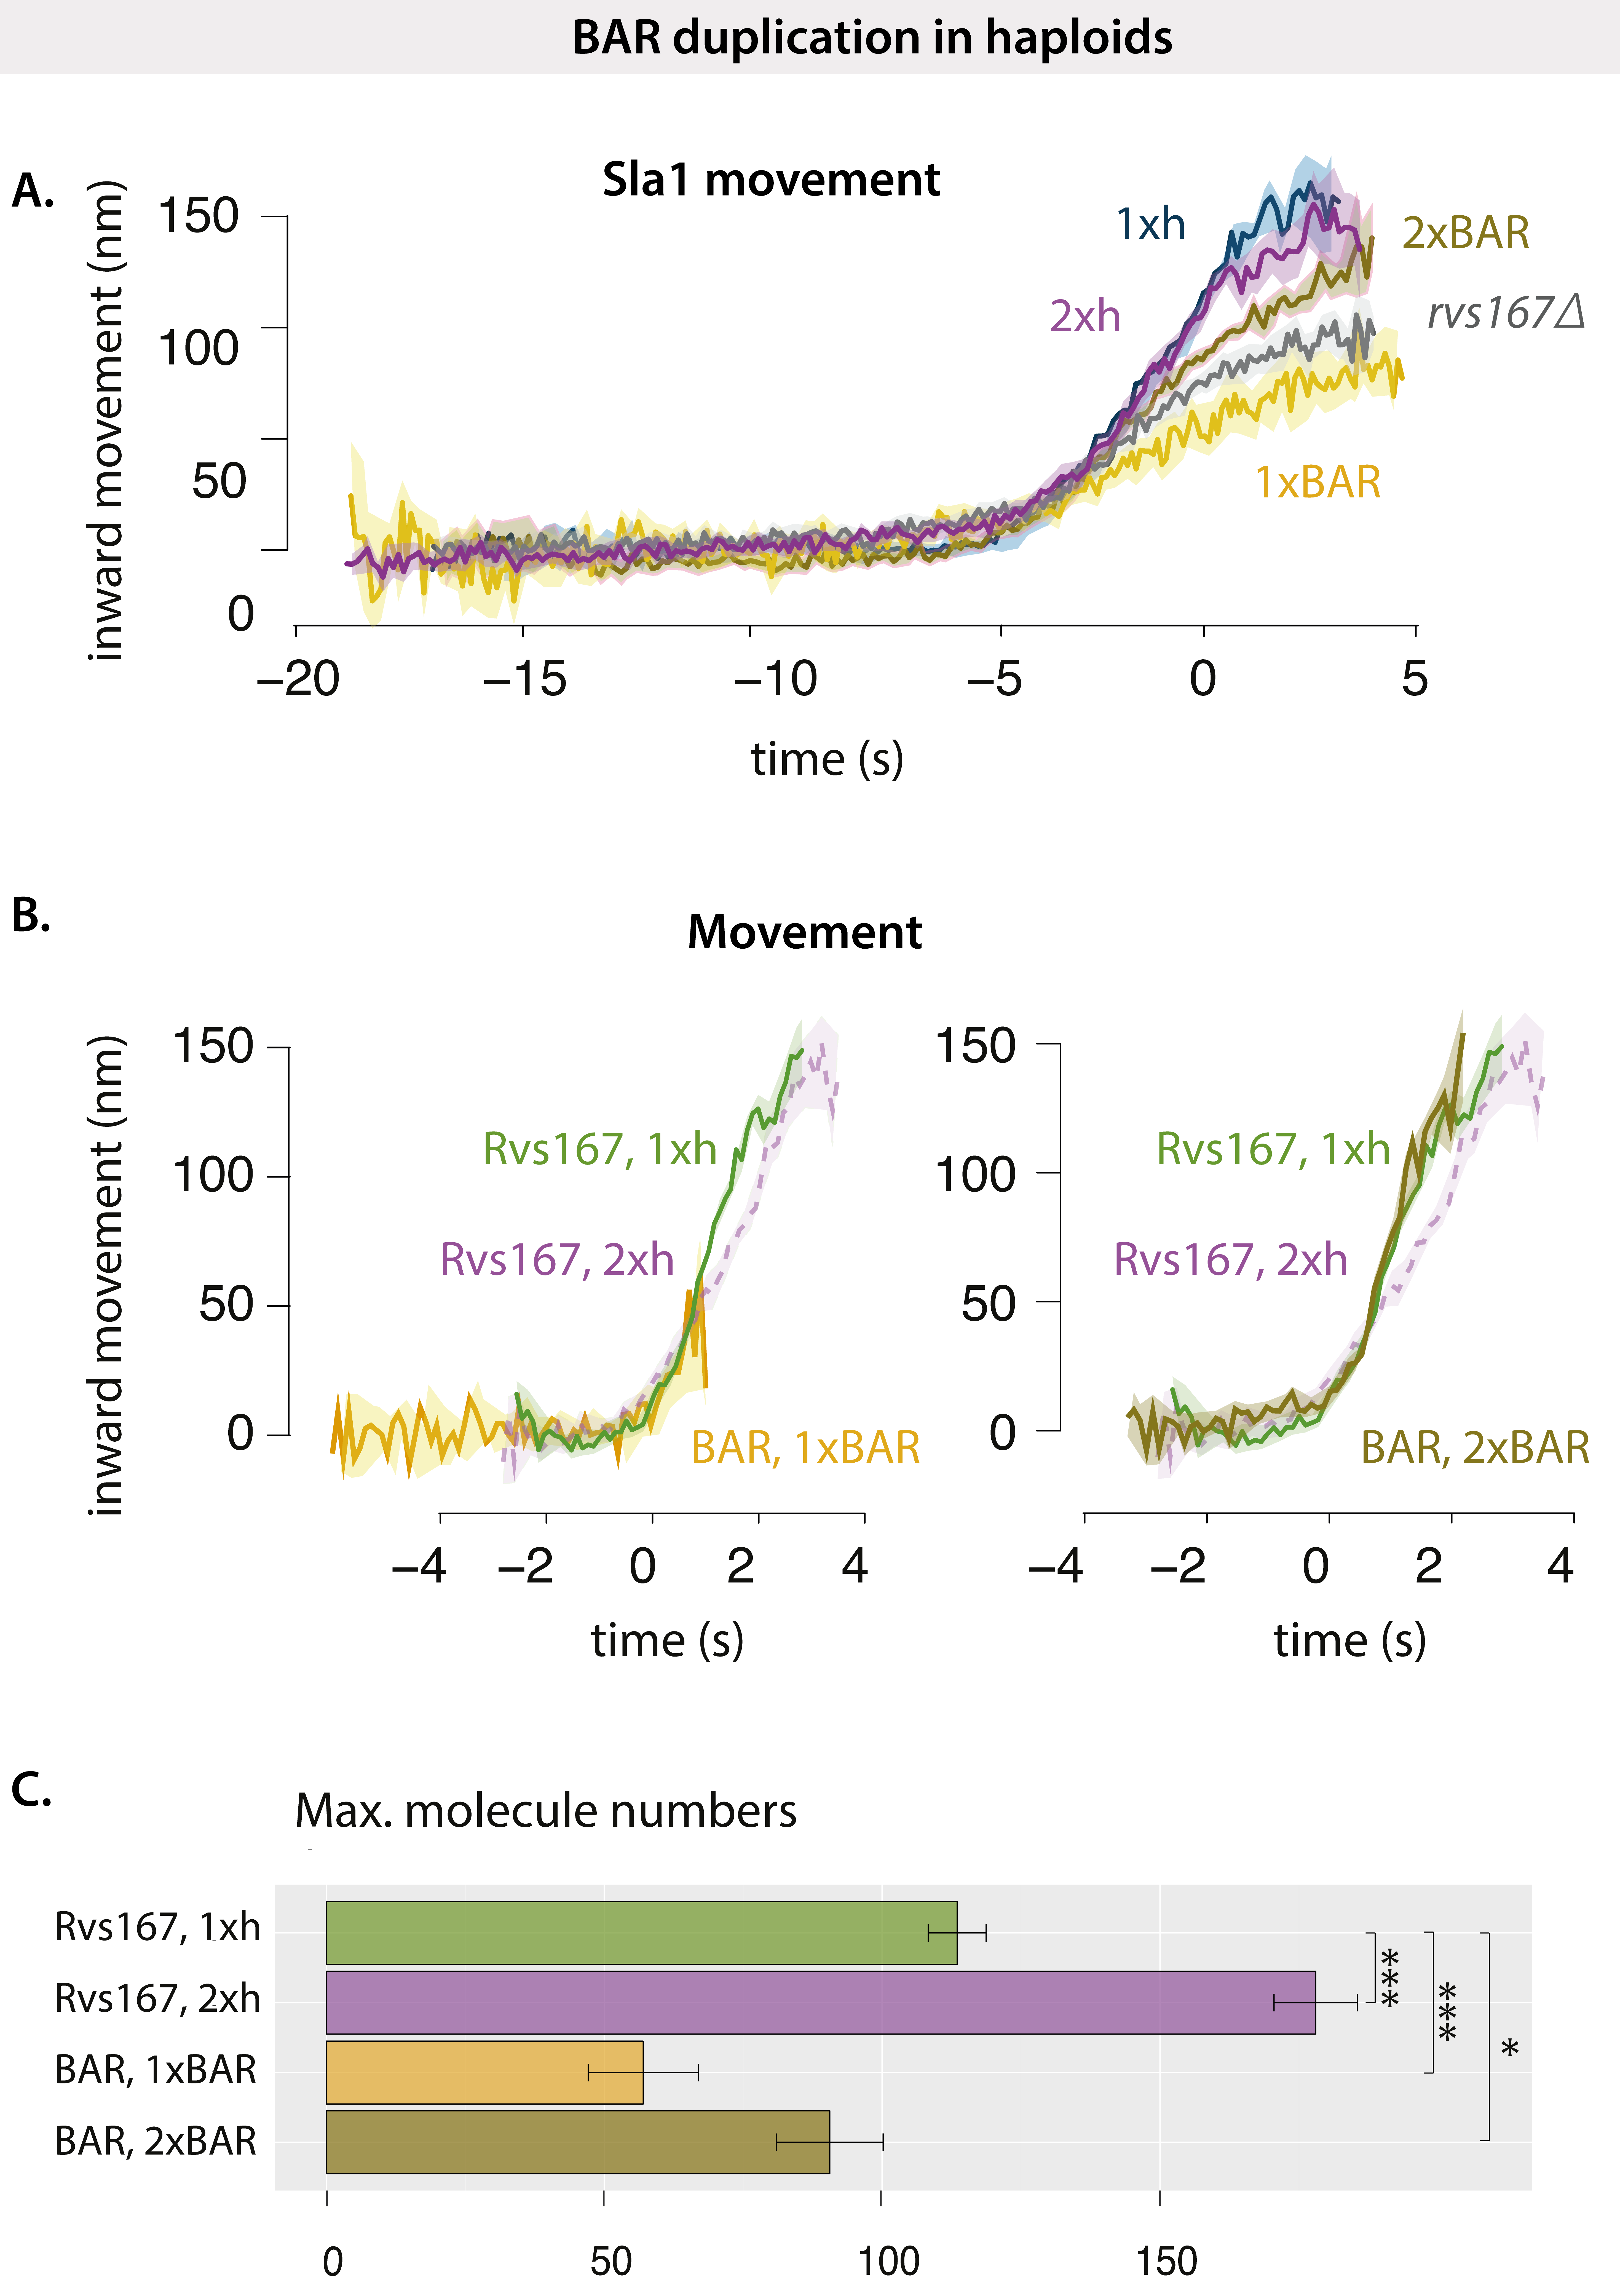
\includegraphics[width=21cm,height=21 cm,keepaspectratio]{figures/results_final/scaffolding_overlaid3}
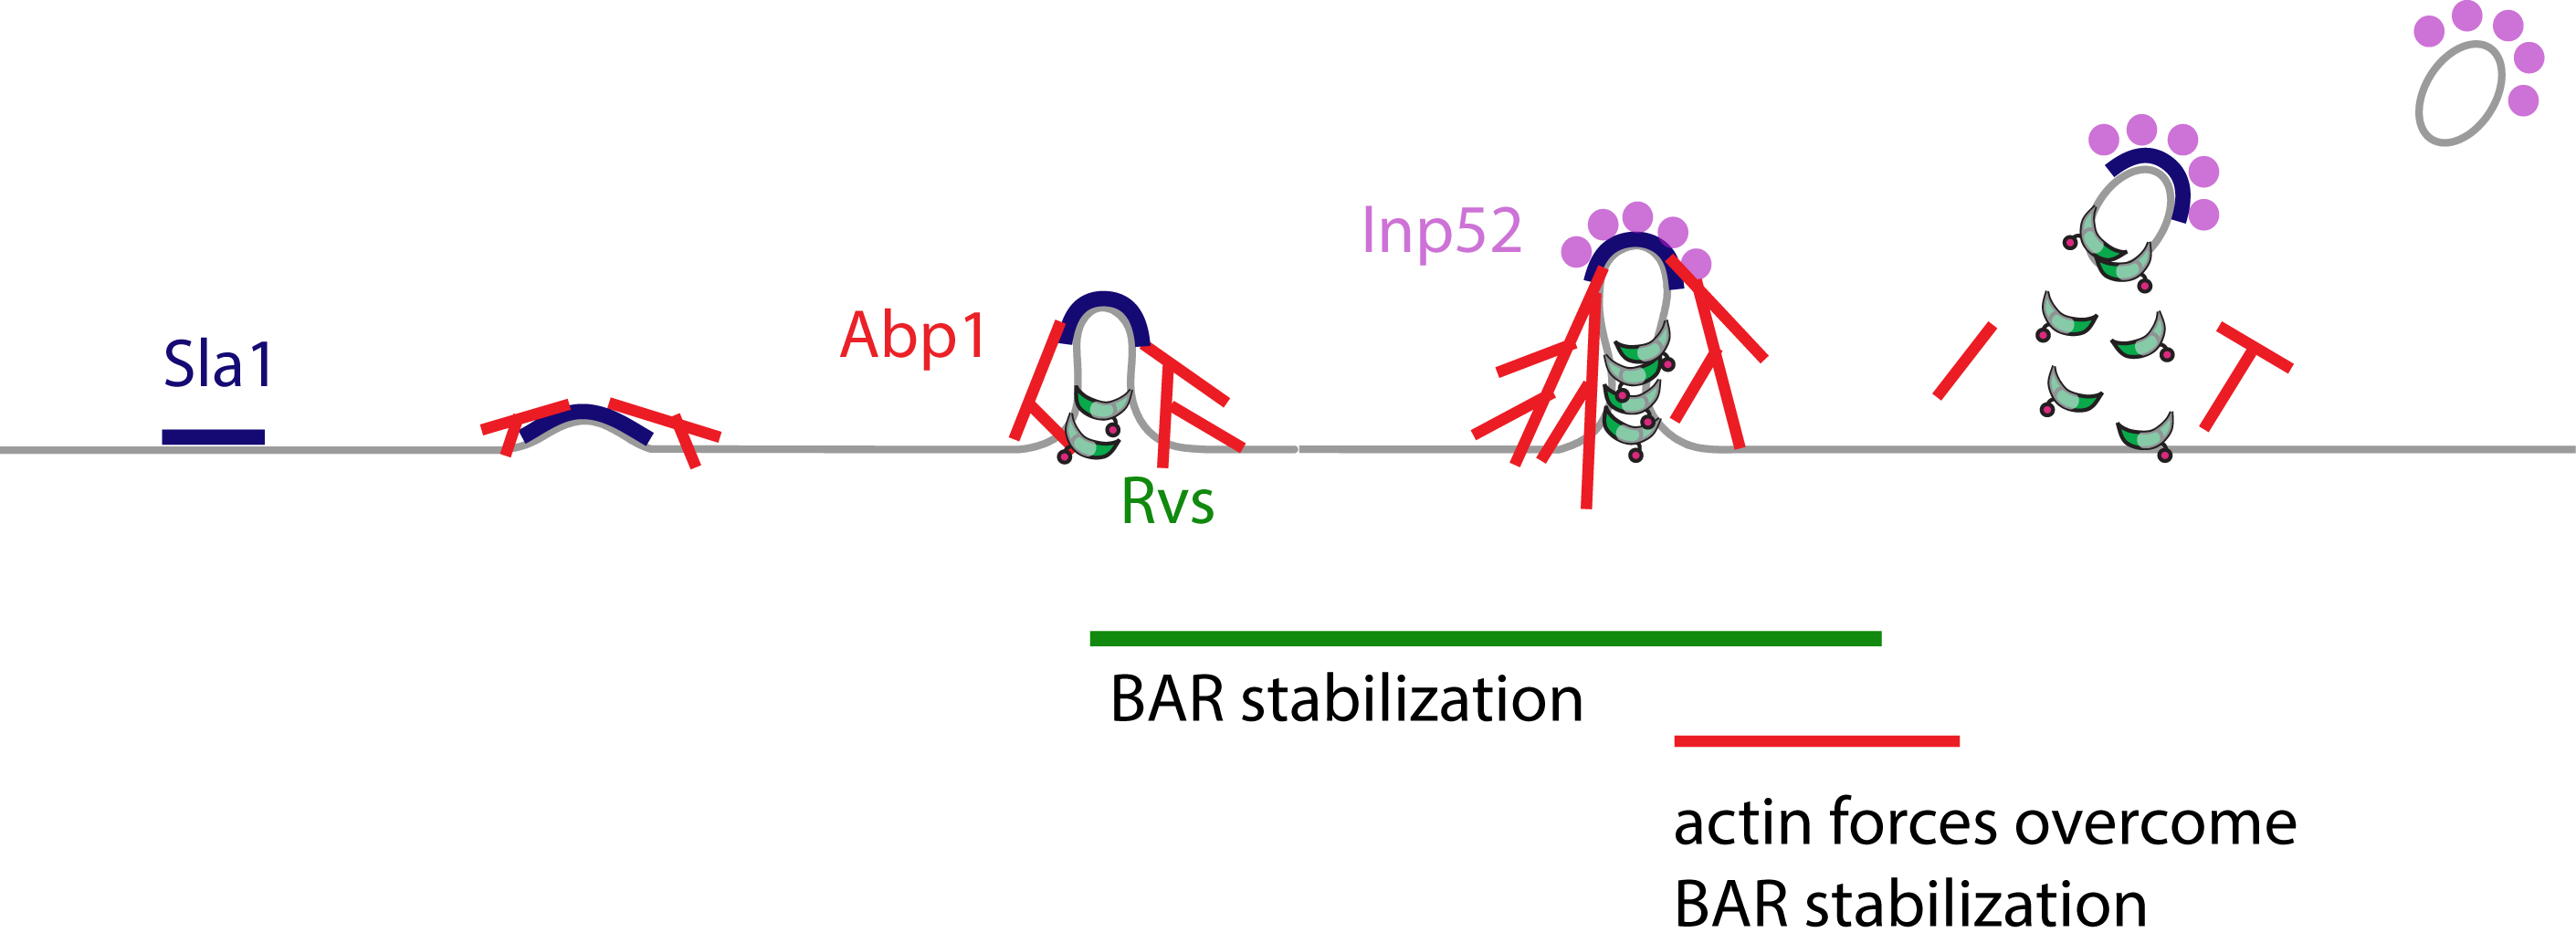
\includegraphics[scale=0.67]{figures/discussion/yeast_schematic_concl2}
	\caption [n]
	{ }
	\label{fig_scaffold}
\end{figure}

%\section{Other potential scission mechanisms and open questions}

%\cite{Dmitrieff2015a}
%clustering induces scission 
%cooperation between lipid hydrolysis and actin forces?


%why these curvatures? specificity from the SH3 domain?
%why does it come off
%regulation of activity? phophorylation/ autoinhibition

